\documentclass{cmc}
\usepackage{makecell}


\begin{document}

\pagestyle{fancy}
\lhead{\textit{\textbf{Computational Motor Control, Spring 2020} \\
    Final project, Lab 8, GRADED}} \rhead{Zhou Xiao \\ Lu Xiaolong \\ Joseph Al Aaraj}

\section*{Student names: Zhou Xiao, Lu Xiaolong, Joseph Al Aaraj}

\textit{Instructions: Update this file (or recreate a similar one, e.g.\ in
  Word) to prepare your answers to the questions. Feel free to add text,
  equations and figures as needed. Hand-written notes, e.g.\ for the development
  of equations, can also be included e.g.\ as pictures (from your cell phone or
  from a scanner).  \textbf{\corr{This lab is graded.}} and needs to be
  submitted before the \textbf{\corr{Deadline : Wednesday 27-05-2020 23:59. You
      only need to submit one final report for all of the following exercises
      combined henceforth.}} Please submit both the source file (*.doc/*.tex)
  and a pdf of your document, as well as all the used and updated Python
  functions in a single zipped file called
  \corr{final\_report\_name1\_name2\_name3.zip} where name\# are the team
  member’s last names.  \corr{Please submit only one report per team!}}
\\

\section*{Swimming with Salamandra robotica – CPG Model}
\label{sec:exploring-swimming}

In this project you will control a salamander-like robot Salamandra
robotica II for which you will use Python and the PyBullet physics
engine. Now you have an opportunity to use what you’ve learned until
now to make the robot swim and eventually walk. In order to do this,
you should implement a CPG based swimming controller, similarly to the
architecture shown in Figure~\ref{fig:controller-model}.

The project is based on the research of \cite{Crespi2013},
\cite{Karakasiliotis2013} and \cite{ijspeert2007swimming}. It is strongly
recommended to review \cite{ijspeert2007swimming} and its supplementary material
provided on the Moodle. You will be tasked with replicating and
studying the Central Pattern Generator (CPG).

\corr{\textit{NOTE : }} The session this week will be an introduction to the
final project. You will be installing the PyBullet physics engine will and get
to familiarise with it. You will start implementing the CPG network which will
eventually control the robot.

\begin{figure}[h]
  \centering
  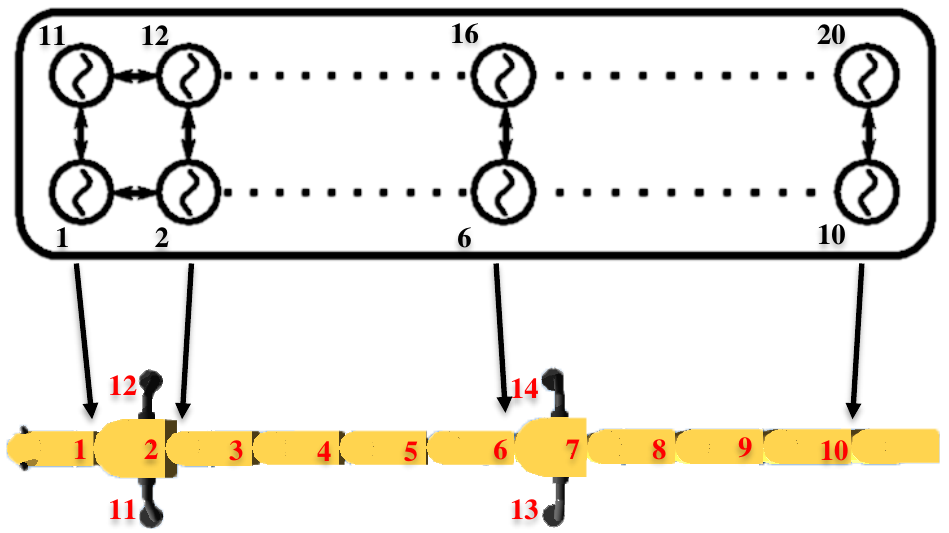
\includegraphics[width=0.5\textwidth]{figures/model_controller.png}
  \caption[Controller model]{A double chain of oscillators controlling
    the robot’s spine.}
  \label{fig:controller-model}
\end{figure}

\begin{figure}[ht]
  \centering 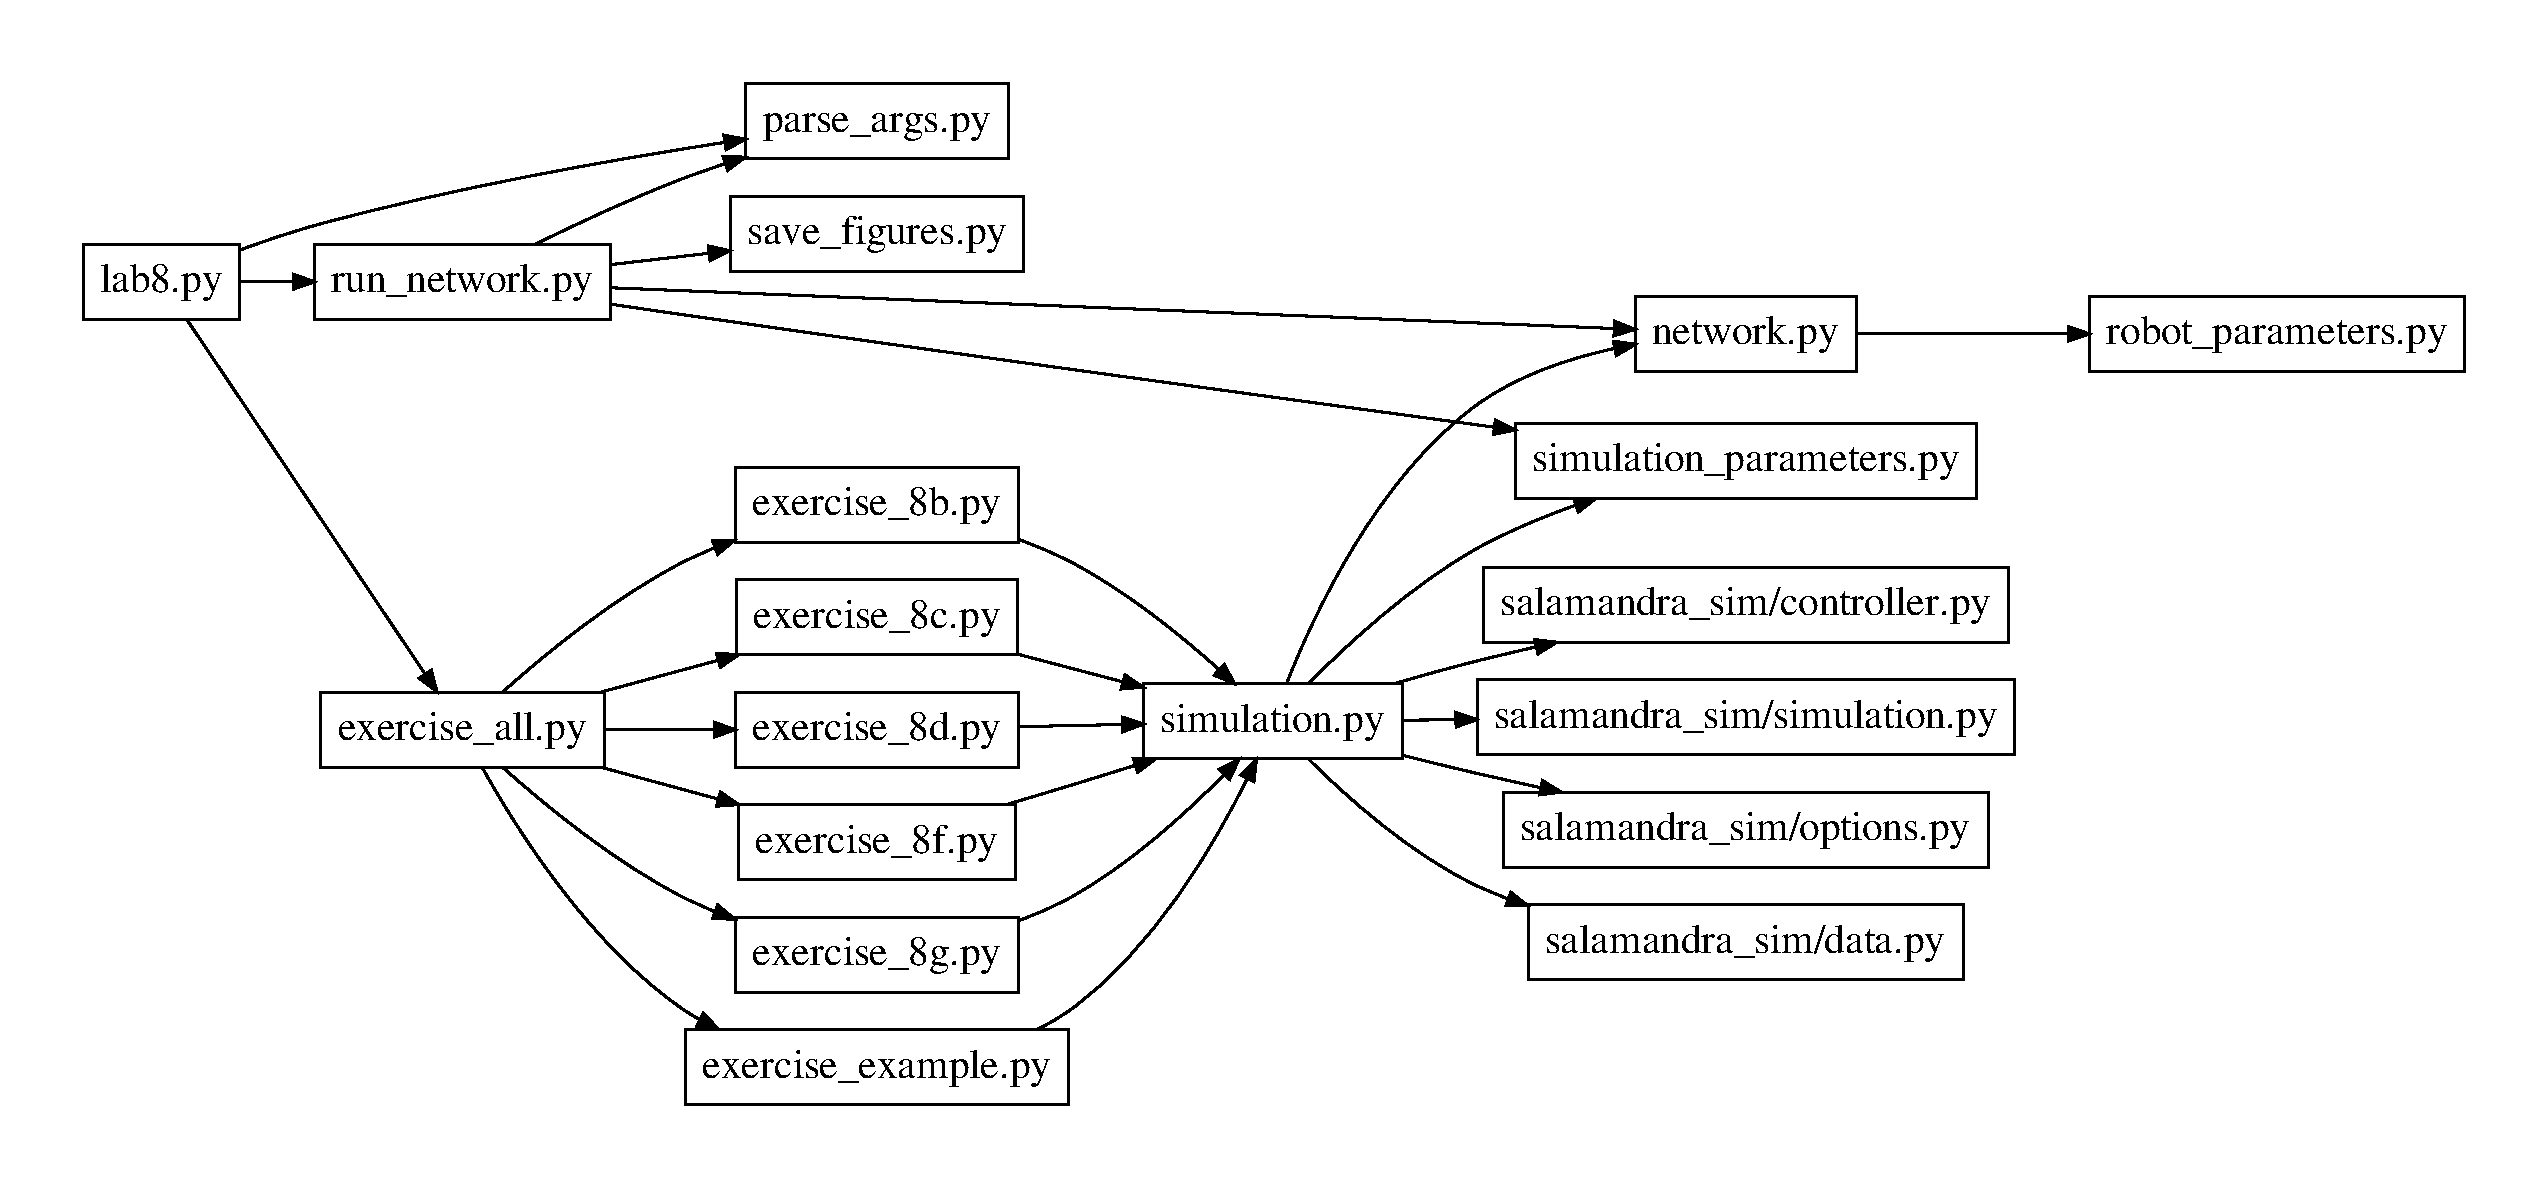
\includegraphics[width=1.0\textwidth]{figures/files}
  \caption{\label{fig:files} Exercise files dependencies. In this lab, you will
    be modifying \fileref{run\_network.py}, \fileref{network.py},
    \fileref{robot\_parameters.py} and \fileref{simulation\_parameters.py}}
\end{figure}

% \newpage

\subsection*{Code organization}
\label{subsec:code}

\begin{itemize}
\item \corr{\textbf{exercise\_all.py}} - A convenient file for running all
  exercises. Note you can also run the simulations in parallel by activating
  \texttt{parallel=True}. \textit{You do not need to modify this file.}
\item \corr{\textbf{network.py}} - This file contains the different classes and
  functions for the CPG network and the Ordinary Differential Equations
  (ODEs). You can implement the network parameters and the ODEs here. Note that
  some parameters can be obtained from pythonController.py to help you control
  the values.
\item \corr{\textbf{robot\_parameters.py}} - This file contains the different
  classes and functions for the parameters of the robot, including the CPG
  network parameters. You can implement the network parameters here. Note that
  some parameters can be obtained from SimulationParameters class in
  \corr{simulation\_parameters.py} and sent by \corr{exercise\_\#.py} to help
  you control the values (refer to example).
\item \corr{\textbf{simulation\_parameters.py}} - This file contains the
  SimulationParameters class and is provided for convenience to send parameters
  to the setup of the network parameters in \corr{robot\_parameters.py}. All the
  values provided in SimulationParameters are actually logged in
  \corr{cmc\_robot.py}, so you can also reload these parameters when analyzing
  the results of a simulation.
\item \corr{\textbf{run\_network.py}} - By running the script from Python,
  PyBullet will be bypassed and you will run the network without a physics
  simulation. Make sure to use this file for question 8a to help you with
  setting up the CPG network equations and parameters and to analyze its
  behavior. This is useful for debugging purposes and rapid controller
  development since running the Pybullet simulation takes more time.
\item \corr{\textbf{parse\_args.py}} - Used to parse command line arguments for
  run\_network.py and plot\_results.py and determine if plots should be shown or
  saved directly. \textit{You do not need to modify this file.}
\item \corr{\textbf{save\_figures.py}} - Contains the functions to automatically
  detect and save figures. \textit{You do not need to modify this file.}
\item \corr{\textbf{test\_sr2.py}} - This is a file to verify that Pybullet was
  installed correctly. It is important to make sure that this file works as it
  will be necessary for the project. \textit{You do not need to modify this
    file.}
\item \corr{\textbf{exercise\_example.py}} - Contains the example code structure
  to help you familiarize with the other exercises. \textit{You do not need to
    modify this file.}
\item \corr{\textbf{exercise\_\#.py}} - To be used to implement and answer the
  respective exercise questions. Note that \corr{exercise\_example.py} is
  provided as an example to show how to run a parameter sweep. Note that network
  parameters can be provided here.
\item \corr{\textbf{exercise\_all.py}} - A convenient file for running different
  exercises depending on arguments. See \corr{\textbf{lab8.py}} for an example
  on how to call it. \textit{You do not need to modify this file.}
\item \corr{\textbf{simulation.py}} A simulation function is provided for
  convenience to easily run simulations with different parameters. You are free
  to implement other functions to run simulations as necessary.
\item \corr{\textbf{plot\_results.py}} - Use this file to load and plot the
  results from the simulation. This code runs with the original pythonController
  provided.
\end{itemize}

% \newpage

\section*{Prerequisites}
To have all the necessary python packages necessary to complete the
final project, do the following.

Clone the latest version of the exercise repository. Navigate to the
location of your repository in the terminal and execute the following,

\begin{lstlisting}[language=Bash]
  >> pip install -r requirements.txt
\end{lstlisting}

\subsection*{Running the simulation}
You can run a simulation example with \corr{\textbf{exercise\_example.py}}. You
should see the Salamandra robotica model floating on the water. At this point
you can now start to work on implementing your exercises.

\newpage

\section*{Questions}

The exercises are organized such that you will have to first implement the
oscillator network model in \corr{run\_network.py} code and analyze it before
connecting it to the body in the physics simulation.  Exercise 8a describes the
questions needed to implement the oscillator models. After completing exercise
8a you should have an oscillator network including both the spinal CPG and limb
CPG. Using the network implemented in exercise 8a you can explore the swimming,
walking and transition behaviors in the Salamandra robotica II model using the
pybullet simulation and complete exercises 8b to 8g.

\subsection*{8a. Implement a double chain of oscillators along with
  limb CPG's}
\label{sec:implement-chain}

Salamandra robotica has 10 joints along its spine and 1 joint for each
limb. The controller is defined as

\begin{equation}
  \label{eq:dphase}
  \dot{\theta}_i = 2 \pi f + \sum_j r_j w_{ij} sin(\theta_j - \theta_i - \phi_{ij})
\end{equation}

\begin{equation}
  \label{eq:dr}
  \dot{r}_i = a (R_i - r_i)
\end{equation}

\begin{equation}
  \label{eq:output}
  q_i = r_i(1 + cos(\theta_i)) - r_{i+10}(1 + cos(\theta_{i+10})) \text{ if body joint}
\end{equation}

with $ \theta_i $ the oscillator phase, f the frequency, $ w_{ij} $ the coupling
weights, $ \phi_{ij} $ the nominal phase lag (phase bias), $ r_i $ the
oscillator amplitude, $ R_i $ the nominal amplitude, $ a $ the convergence
factor and $ q_i $ the spinal joint angles. For more information, please refer
to \cite{ijspeert2007swimming}. Also note how these are the same equations,
although Equation \eqref{eq:dr} has been simplified into a first order ODE in
order to simplify the implementation in this project.


\begin{enumerate}
\item Implement the double chain oscillator model using the functions
  \fileref{network.py::network\_ode}. Test your implementation by running the
  network using \fileref{run\_network.py}. For the network parameters check
  lecture slides (pay attention to different number of segments). You can also
  find more information in \cite{ijspeert2007swimming} (especially in the
  supplementary material). You can set all the network parameters in the
  \fileref{robot\_parameters.py::RobotParameters}. To facilitate your work, you
  could start by only implementing the network for the body oscillators
  ($i=[0, ..., 19]$) and ignoring the leg oscillators ($i=[20, ..., 23]$). Refer
  to \corr{network::RobotState} and
  \corr{robot\_parameters.py::}\-\corr{RobotParameters} for the dimensions of
  the state and the network parameters respectively.

\item Implement the output of your CPG network to generate the spinal joint
  angles according to equation \ref{eq:output}. Implement this in the function
  \fileref{network.py::motor\_output}. Verify your implementation in by running
  the Python file \fileref{run\_network.py}.


\item Implement a drive and show that your network can generate swimming and
  walking patterns similarly to \cite{ijspeert2007swimming}. Try to reproduce
  the plots in \ref{fig:science_oscillator_patterns} and
  \ref{fig:science_oscillator_properties}


  \textbf{Hint:} The state for the network ODE is of size 48 where the first 24
  elements correspond to the oscillator phases $\theta_i$ of the oscillators and
  the last 24 elements correspond to the amplitude $r_i$. The initial state is
  set in the init of \corr{network.py::SalamanderNetwork}.
\end{enumerate}

\begin{figure}[H]
  \centering
  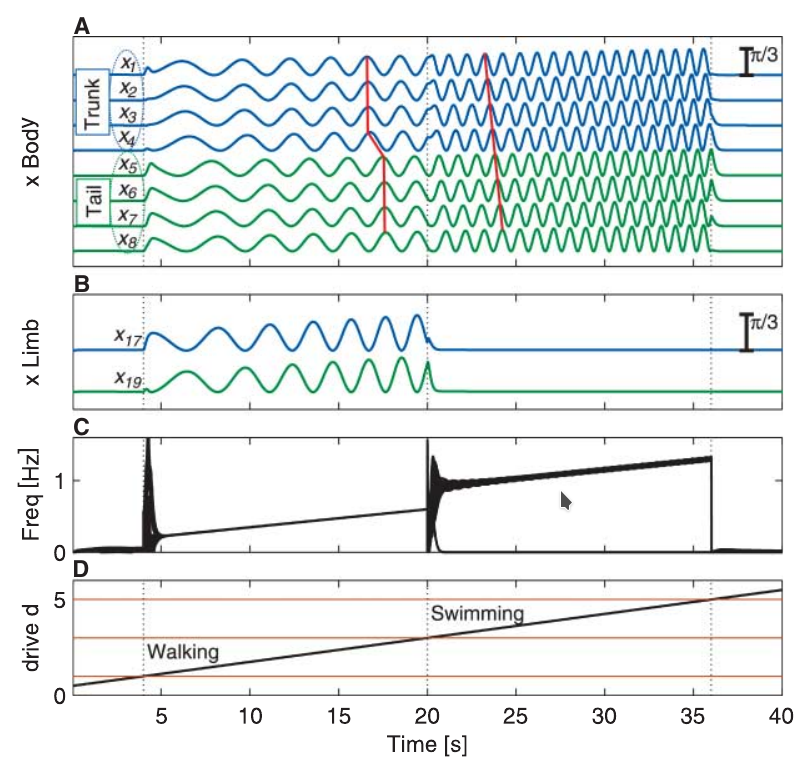
\includegraphics[width=0.7\textwidth]{figures/science_oscillator_patterns}
  \caption{Oscillator patterns from \cite{ijspeert2007swimming}, see
    \cite{ijspeert2007swimming} for details}
  \label{fig:science_oscillator_patterns}
\end{figure}

\begin{figure}[H]
  \centering
  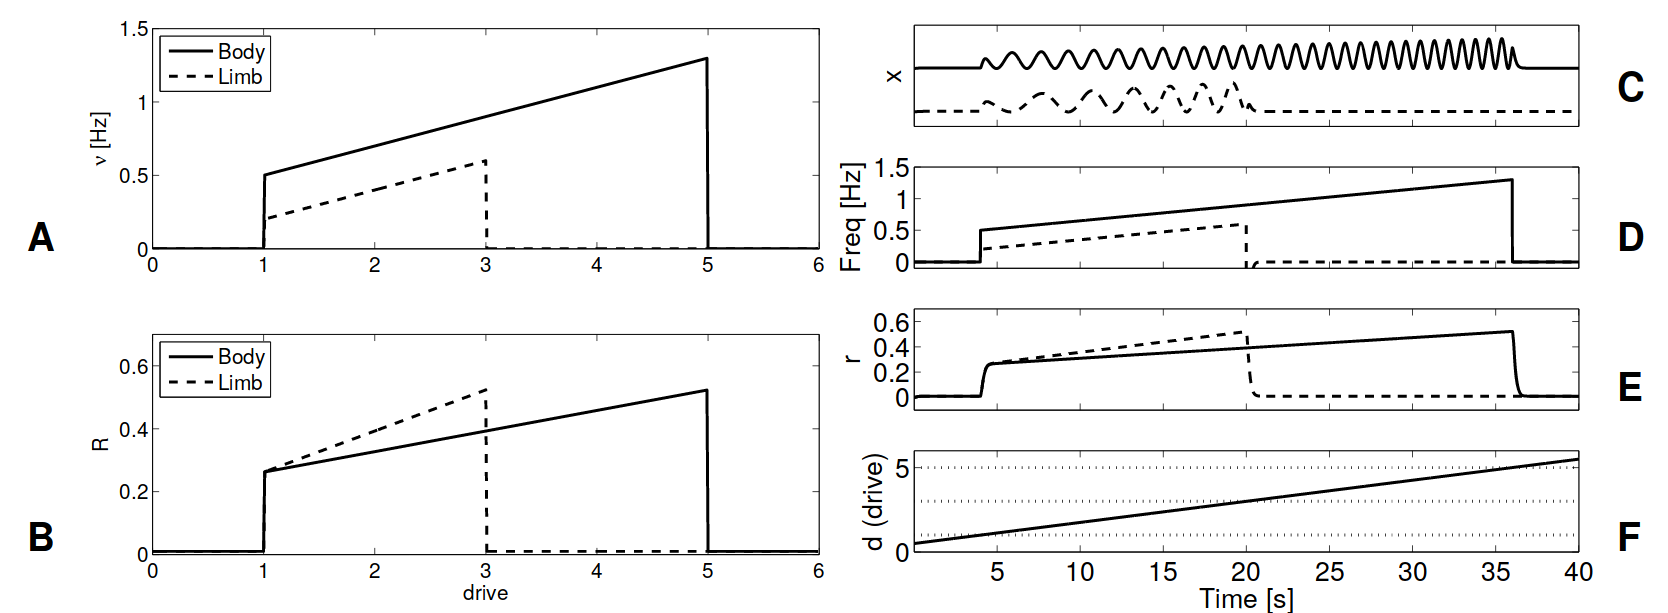
\includegraphics[width=1.0\textwidth]{figures/science_oscillator_properties}
  \caption{Oscillator properties from \cite{ijspeert2007swimming} supplementary
    material, see \cite{ijspeert2007swimming} for details}
  \label{fig:science_oscillator_properties}
\end{figure}

% 在这儿写

\begin{figure}[H]
\centering
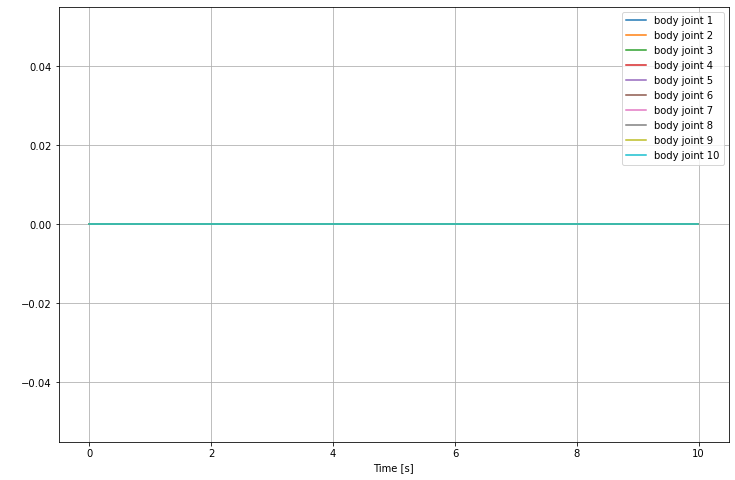
\includegraphics[height=0.3\columnwidth]{figures/8a_d05_spine.png}
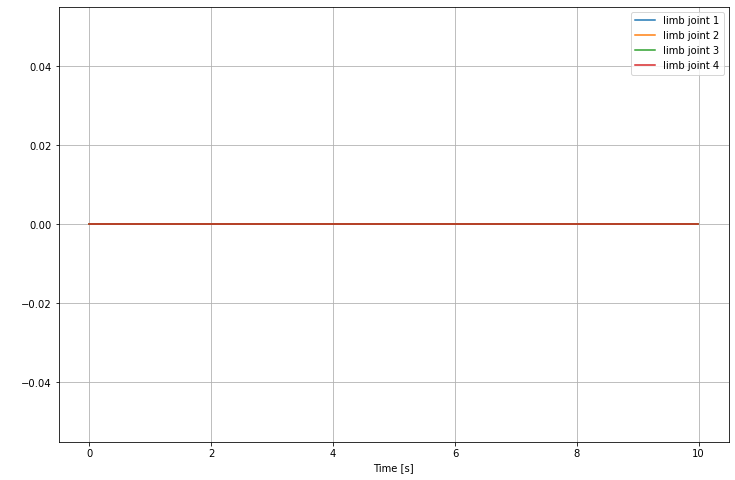
\includegraphics[height=0.3\columnwidth]{figures/8a_d05_limb.png}
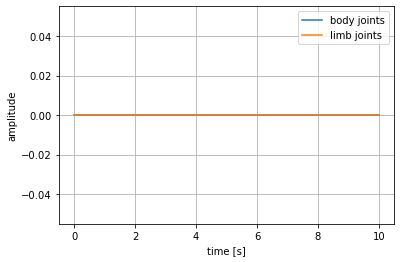
\includegraphics[height=0.3\columnwidth]{figures/8a_d05_amp.png}
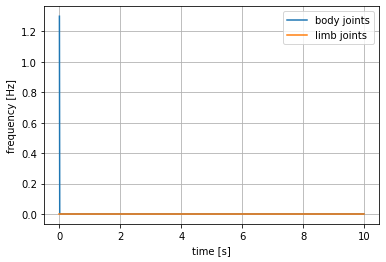
\includegraphics[height=0.3\columnwidth]{figures/8a_d05_freq.png}
\caption{Oscillation properties of walking with drive=0.5 in our simulation}
\label{a0}
\end{figure}


\begin{figure}[H]
\centering
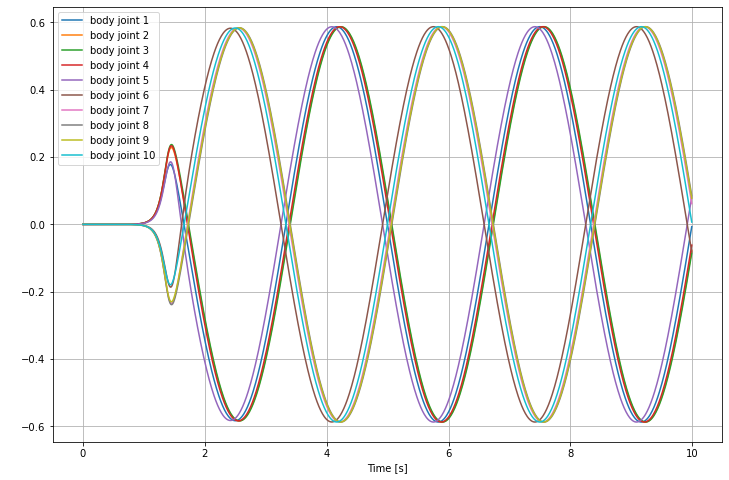
\includegraphics[height=0.3\columnwidth]{figures/8a_d15_spine.png}
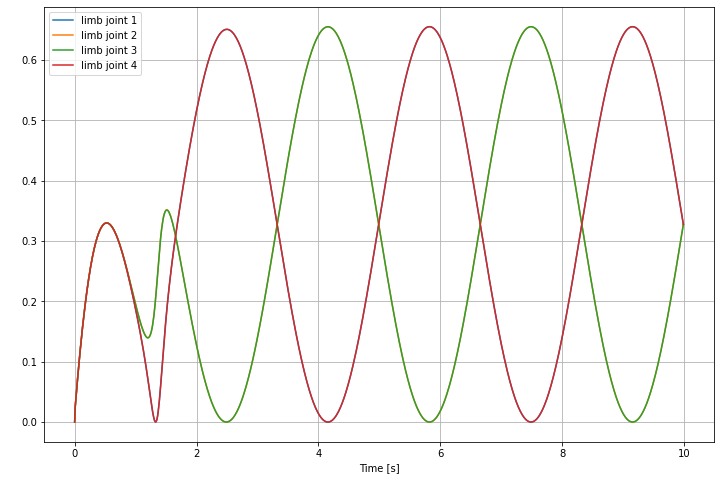
\includegraphics[height=0.3\columnwidth]{figures/8a_d15_limb.png}
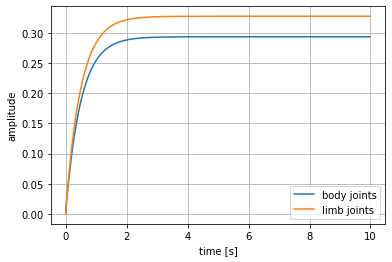
\includegraphics[height=0.3\columnwidth]{figures/8a_d15_amp.png}
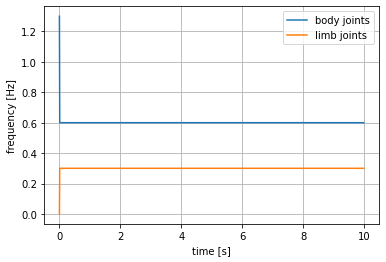
\includegraphics[height=0.3\columnwidth]{figures/8a_d15_freq.png}
\caption{Oscillation properties of swimming with drive=1.5 in our simulation}
\label{a1}
\end{figure}

\begin{figure}[H]
\centering
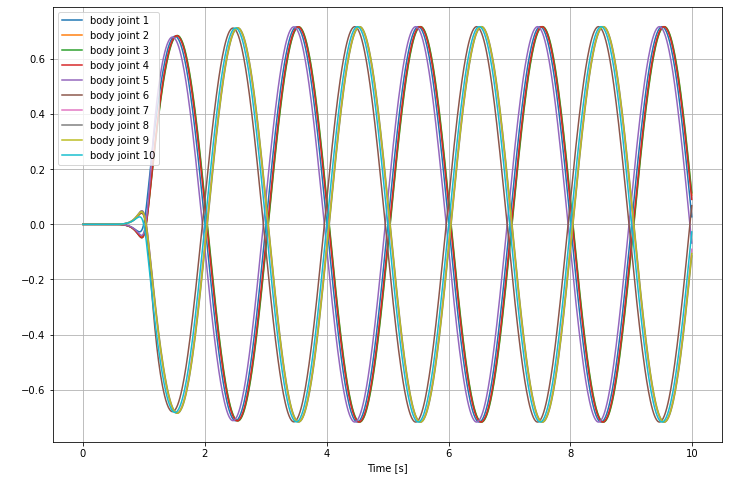
\includegraphics[height=0.3\columnwidth]{figures/8a_d25_spine.png}
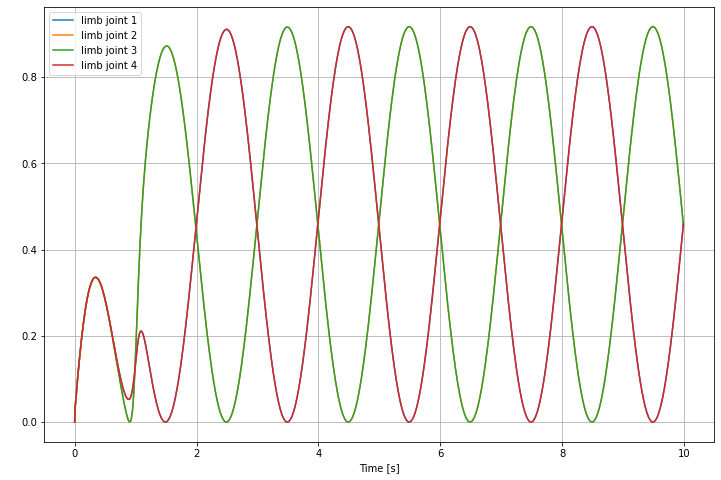
\includegraphics[height=0.3\columnwidth]{figures/8a_d25_limb.png}
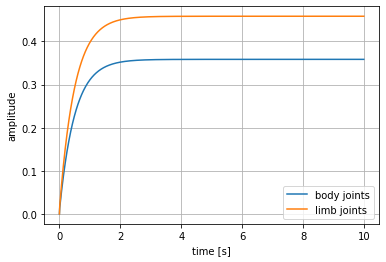
\includegraphics[height=0.3\columnwidth]{figures/8a_d25_amp.png}
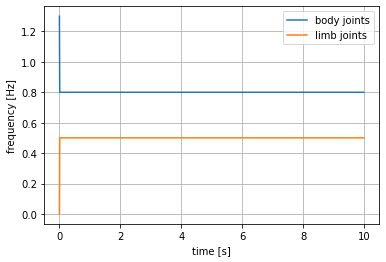
\includegraphics[height=0.3\columnwidth]{figures/8a_d25_freq.png}
\caption{Oscillation properties of swimming with drive=2.5 in our simulation}
\label{a2}
\end{figure}

\begin{figure}[H]
\centering
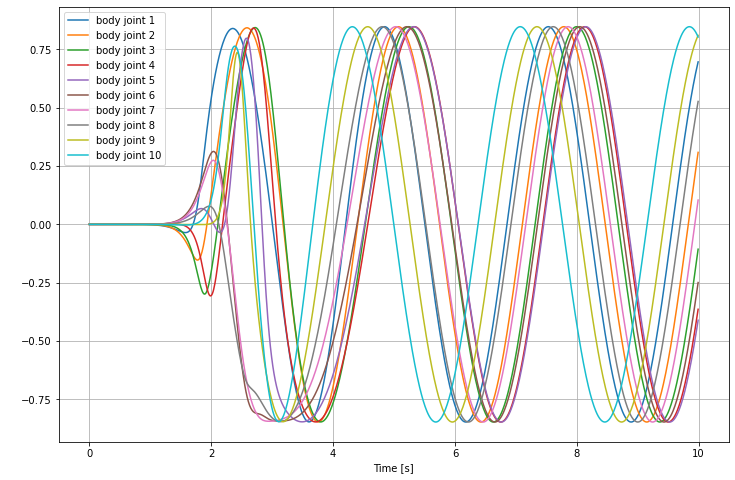
\includegraphics[height=0.3\columnwidth]{figures/8a_d35_spine.png}
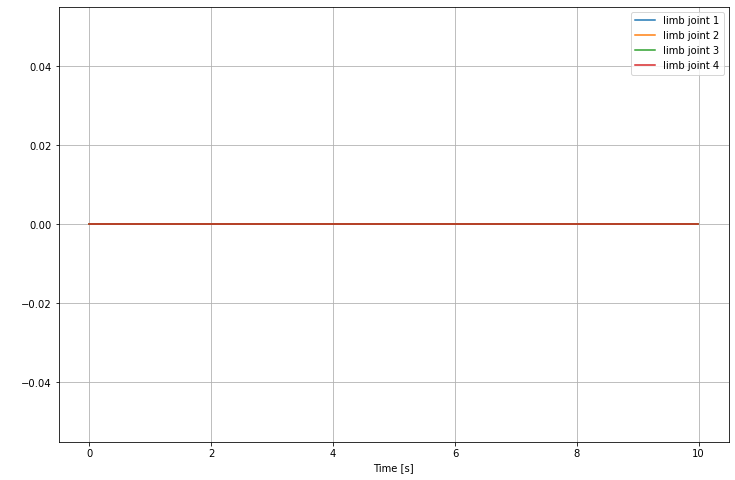
\includegraphics[height=0.3\columnwidth]{figures/8a_d35_limb.png}
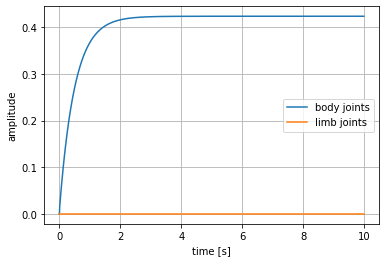
\includegraphics[height=0.3\columnwidth]{figures/8a_d35_amp.png}
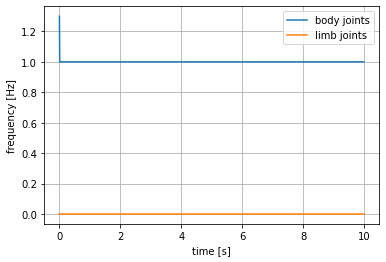
\includegraphics[height=0.3\columnwidth]{figures/8a_d35_freq.png}
\caption{Oscillation properties of walking with drive=3.5 in our simulation}
\label{a3}
\end{figure}

\begin{figure}[H]
\centering
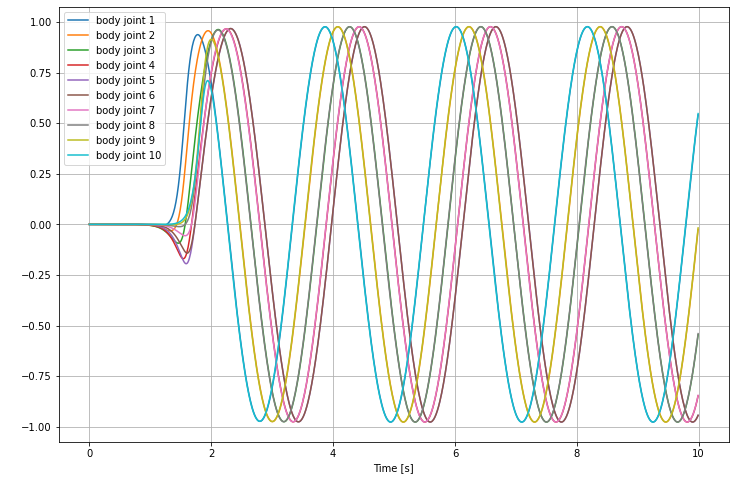
\includegraphics[height=0.3\columnwidth]{figures/8a_d45_spine.png}
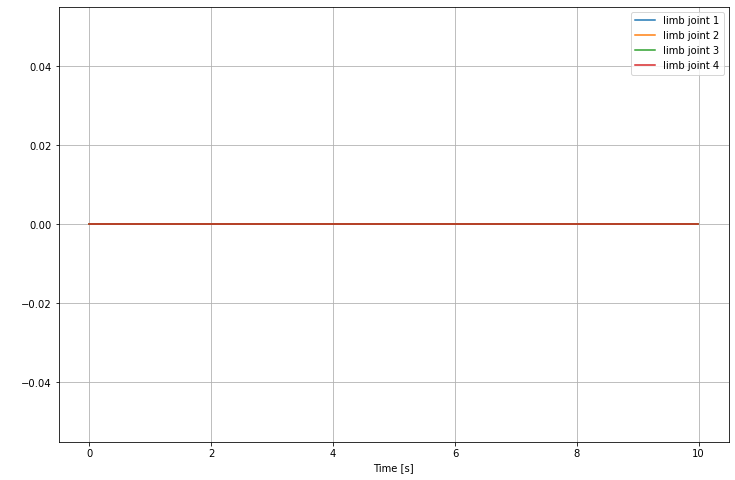
\includegraphics[height=0.3\columnwidth]{figures/8a_d45_limb.png}
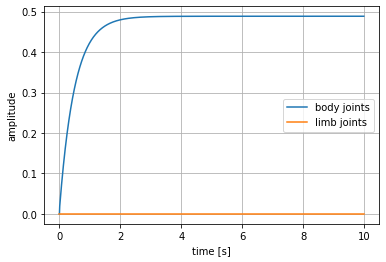
\includegraphics[height=0.3\columnwidth]{figures/8a_d45_amp.png}
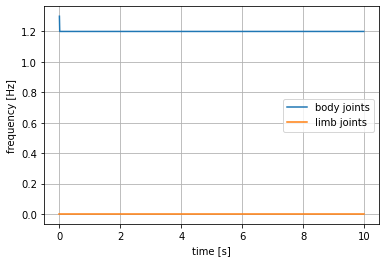
\includegraphics[height=0.3\columnwidth]{figures/8a_d45_freq.png}
\caption{Oscillation properties of walking with drive=4.5 in our simulation}
\label{a4}
\end{figure}

\begin{figure}[H]
\centering
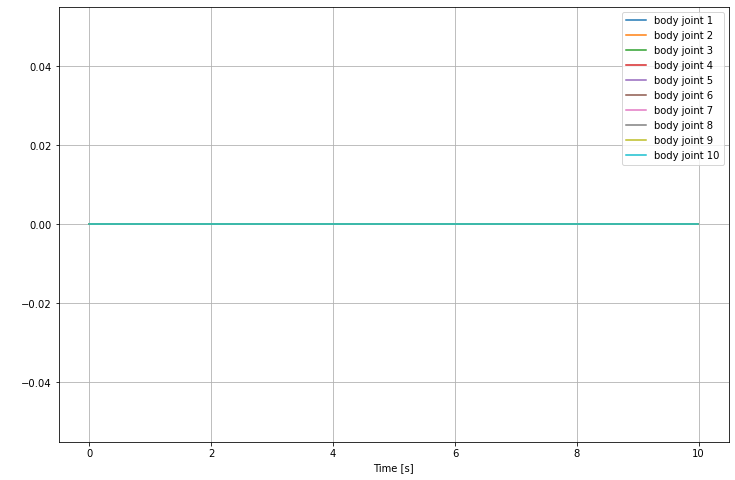
\includegraphics[height=0.3\columnwidth]{figures/8a_d55_spine.png}
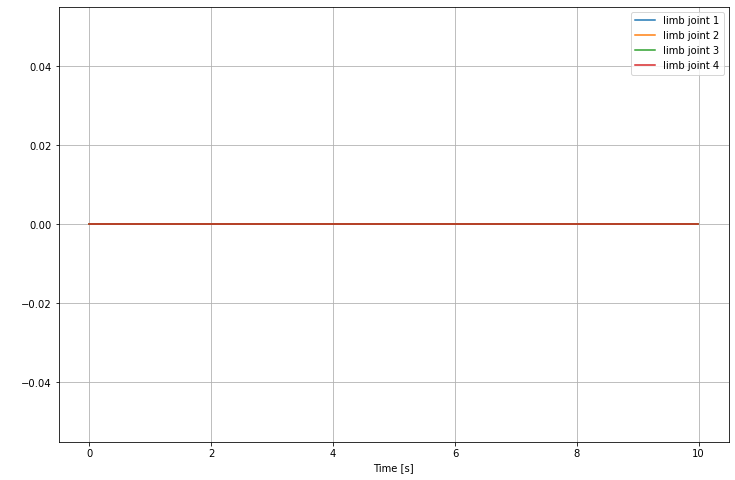
\includegraphics[height=0.3\columnwidth]{figures/8a_d55_limb.png}
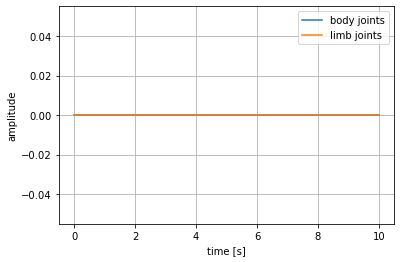
\includegraphics[height=0.3\columnwidth]{figures/8a_d55_amp.png}
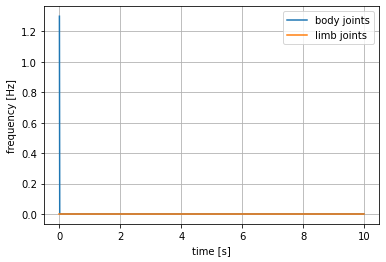
\includegraphics[height=0.3\columnwidth]{figures/8a_d55_freq.png}
\caption{Oscillation properties of walking with drive=5.5 in our simulation}
\label{a5}
\end{figure}

\begin{figure}[H]
\centering
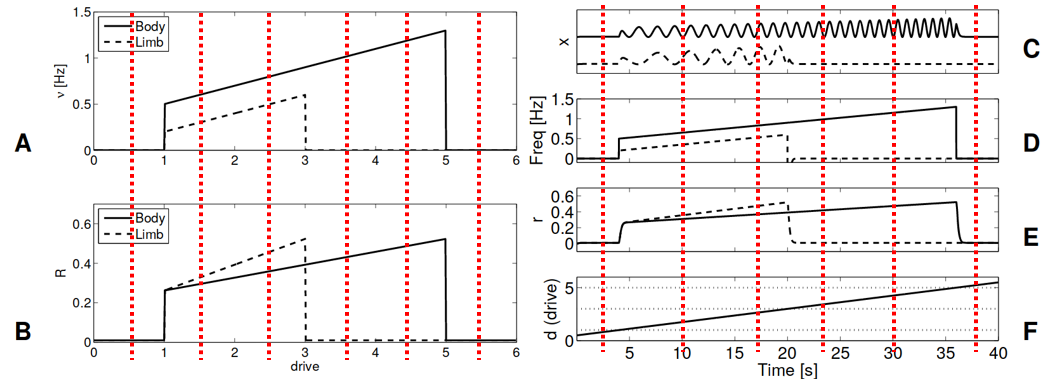
\includegraphics[height=0.3\columnwidth]{figures/8a_ref.png}
\caption{Highlight of oscillation properties with drive=0.5, 1.5 , 2.5 , 3.5 , 4.5, 5.5 in complementary material}
\label{a_ref}
\end{figure}

\begin{figure}[H]
\centering
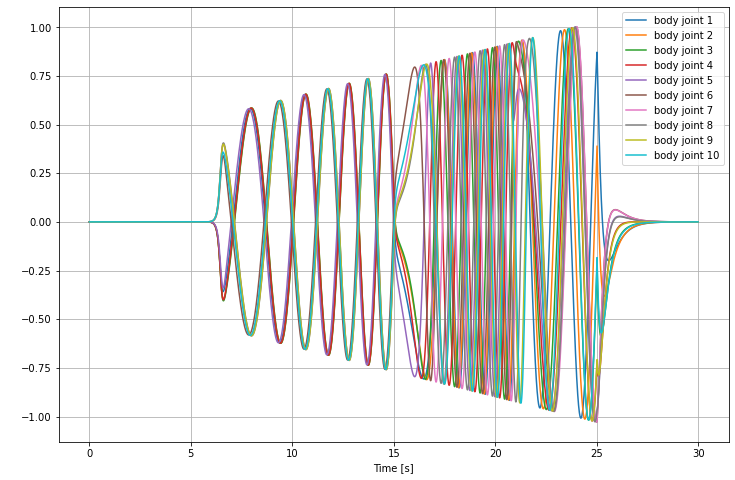
\includegraphics[height=0.3\columnwidth]{figures/8a_spine.png}
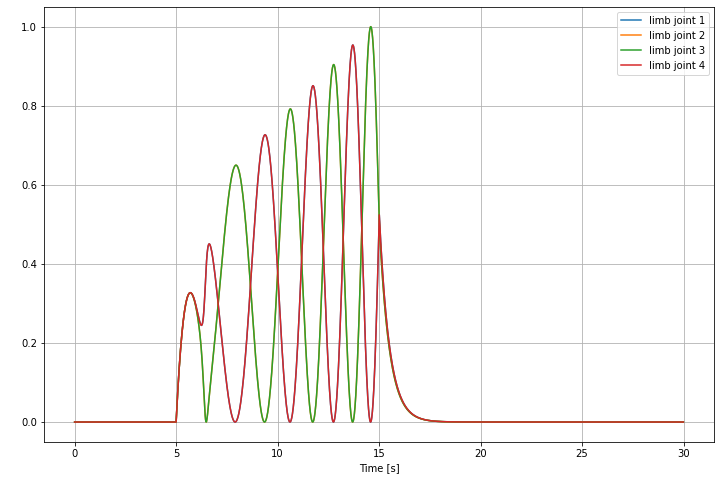
\includegraphics[height=0.3\columnwidth]{figures/8a_limb.png}
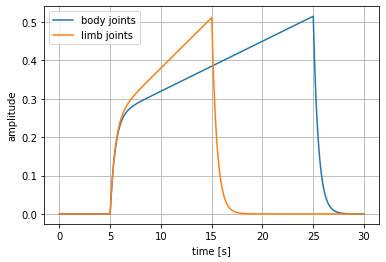
\includegraphics[height=0.3\columnwidth]{figures/8a_amp.png}
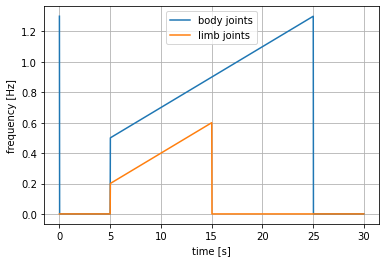
\includegraphics[height=0.3\columnwidth]{figures/8a_freq.png}
\caption{Oscillation properties when drive increases from 0 to 6 linearly within 30 seconds.}
\label{a_f}
\end{figure}

Here we visualize the oscillator performance with different constant values (Figure 5-10) for steady observation, and changing drive (Figure 12) similar to reference plot.

Picture 5-10 show the transition from walking to swimming with different drives. When walking, axial produces standing waves. With the same descending signal, the phase of the output of the four body joints in trunk is the same and that in the tail is also the same but the difference between the the phase of body joint in trunk and that in tail is 180 degrees (Figure 3A). When swimming, axial produces traveling waves, body joints remain constant phase lag along the spinal cord and the relative phase lag between head and tail is usually 100 percentage (Figure 3A).

Figure 4 (left) shows that the limb oscillators oscillate with lower frequencies than body oscillators at the same level of tonic drive d and saturate at with lower drive. While the limb oscillators converge to a higher amplitude than body oscillators at the same level descending drive signal. In our plots all oscillators are driven by the same drive d. Figure 4 (right) gives us the information that the movement of body and limb oscillators (uncoupled) when the drive increases with time. When the drive is lower than the threshold (1), there are no oscillations for both limb and body. When the drive is the larger than the thresholds, slow oscillations can be seen. When the drive d increases from 1.5 to 2.5 (Figure 6-7), the amplitude of both body and limb joints increase and the oscillations of both joints eventually converge to a stable state. We can see from the lower right corner of each graph that body and limb joints frequencies are also increasing but the former is always larger. 

Further increasing the drive d to 3.5 and it's in a swimming pattern, it surpasses the upper threshold of limb oscillators and they are deactivated and we can see the 0 frequencies and amplitudes. While the amplitude and frequency of the body joints continue to increase, and the phase difference all body joints at the same time also increase with respect to the previous 
case. If we further increase the drive to 4.5, it maintains the same trend of variation as in the case of drive d is 3.5.

When the drive d is lower than the lowest threshold of of the body joints (same of the threshold of the limb joints), the body joints and limb joints do not activate(Figure 5). When the drive d is greater than the highest threshold of of the body joints (and, of course,d has already surpassed the highest threshold of the limb joints now), the body joints and limb joints are all at still(Figure 10).

All the above cases of different drive d are marked in Figure 11. And a smooth continuous variation trend of the amplitude and frequency of both body and limb joints with respect to the variation of drive d are shown in Figure 12. Please note that the body and limb oscillators are decoupled. Just by changing the magnitude of the descending signal d (one dimensional signal ), we realized the modulation of the amplitude and frequency of all limb and body joints, that is, the modulation of the gaits, speed etc (very large dimension).

%In the salamandra-robotica robot the legs are simplified to have just one degree of freedom, unlike a real salamanders legs with multiple of degrees of freedom. For the robot the rotating legs are  enough to emulate the swing and stance phase of a gait cycle in a real animal.


\subsection*{8b. Effects of amplitude and phase lags on swimming
  performance}
\label{sec:amplitude-phase-performance}

Now that you have implemented the controller, it is time to run experiments to
study its behaviour. How does phase lag and oscillation amplitude influence the
speed and energy? Use the provided \corr{exercise\_8b.py} to run a grid search
to explore the robot behavior for different combinations of amplitudes and phase
lags. Use \corr{plot\_results.py} to load and plot the logged data from the
simulation. Include 2D/3D plots showing your grid search results and discuss
them. How do your findings compare to the wavelengths observed in the
salamander?

% Run the grid search twice, for frequencies of 1Hz and 2Hz.

\begin{itemize}
\item \textbf{Hint 1:} To use the grid search, check out the example provided in
  \corr{exercise\_example.py}. This function takes the desired parameters as a
  list of SimulationParameters objects (found in
  \corr{simulation\_parameters.py}) and runs the simulation. Note that the
  results are logged as simulation\_\#.h5 in a specified log folder. After the
  grid search finishes, the simulation will close.
\item \textbf{Hint 2:} An example how to load and visualise grid search results
  is already implemented in \corr{plot\_results.py::main()}. Pay attention to
  the name of the folder and the log files you are loading. Before starting a
  new grid search, change the name of the logs destination folder where the
  results will be stored. In case a grid search failed, it may be safer to
  delete the previous logs to avoid influencing new results by mistake.
\item \textbf{Hint 3:} Estimate how long it will take to finish the grid
  search. Our suggestion is to choose wisely lower and upper limits of parameter
  vectors and choose a reasonable number of samples. To speed-up a simulation,
  make sure to run the simulation in fast mode and without GUI as shown in
  \corr{exercise\_example.py} or using \texttt{--fast} and \texttt{--headless}
  in the Python command line (Use \texttt{--help} for more information).
\item \textbf{Hint 4:} Energy can be estimated by integrating the product of
  instantaneous joint velocities and torques. Feel free to propose your own
  energy metrics, just make sure to include the justification.
\end{itemize}


\begin{figure}[H]
\centering
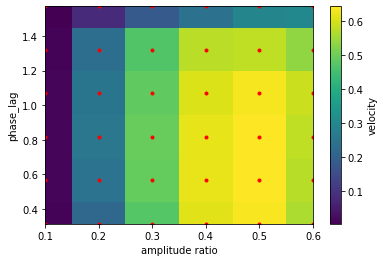
\includegraphics[height=0.3\columnwidth]{figures/8b_v1.png}
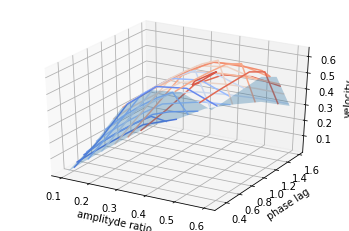
\includegraphics[height=0.3\columnwidth]{figures/8b_v2.png}
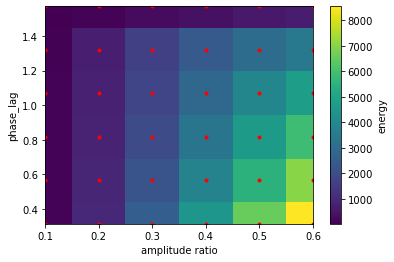
\includegraphics[height=0.3\columnwidth]{figures/8b_e1.png}
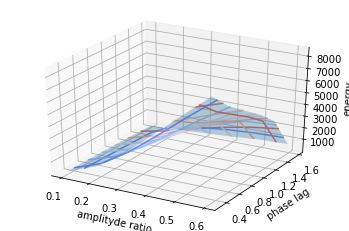
\includegraphics[height=0.3\columnwidth]{figures/8b_e2.png}
\caption{Grid search of phase lag and oscillation amplitude, and their influence on speed (up) and energy (down)}
\label{b}
\end{figure}

In swimming state, the limb of the salamander is deactivated, meaning that it will not affect the whole body. The amplitude and the phase lag are referred to the body oscillators (axial).

Figure 13 is the result of grid search. If we look at the diagram in the upper left corner of the Figure 13, we can find that the smaller the phase lag, the greater the velocity in the case of the same amplitude. When the phase lag is constant, the velocity increases with the increase of the amplitude. However,the velocity achieves the maximum when the amplitude reaches 0.5, and it will decrease with the increase of the amplitude after this point.

In the analysis,  we estimate the energy by integrating the product of instantaneous joint velocities and torques.
In the lower left corner of Figure 13 one can observe how the energy changes with the variation of phase lag and amplitude. The smaller the phase lag, the greater the energy under the same amplitude level. In addition, the larger the amplitude, the greater the energy when the same phase lag appears.

Generally speaking, salamander tends to move in a less energetic manner, where the speed is not necessarily the largest. In our phase lag range, increasing the phase lag can make the energy smaller. When it meets a predator, it moves in the fastest way.  There are three lattice corresponding to the parameters leading to the fastest velocity, but the energy corresponding to the parameters of the three lattice is different. This paved a way for us to reduce the energy at the same speed. We can choose the parameter corresponding to the smallest energy which can still keep a good speed.


Traveling wave has constant phase lag along the spinal cord and the relative phase lag between head and tail is usually 100 percent for any frequency, meaning that the body always makes one complete "S" shaped undulation and the wavelength is constant one body length. While the time needed to complete the entire cycle (traveling wave propagates from the head to tail or from the tail to head) will increase with the increase of the phase lags.
In faster swimming, bursts have higher amplitude, meaning that the muscles will contract more (higher firing rates). In this condition, the bursts are faster, meaning that the bursting frequency is higher. 





\subsection*{8c. Amplitude gradient}
\label{sec:amplitude-gradient}

\begin{enumerate}
\item So far we considered constant undulation amplitudes along the body for
  swimming. Implement a linear distribution of amplitudes along the spine,
  parametrized with two parameters: amplitudes of the first (Rhead) and last
  (Rtail) oscillator in the spine (corresponding to the first and last
  motor). To do so, you can add a parameter amplitudes=[Rhead, Rtail] in
  \corr{simulation\_parameters.py::SimulationParameters}. Don't forget to modify
  \corr{robot\_parameters.py::}\-\corr{RobotParameters::set\_nominal\_amplitudes()}
  and interpolate the amplitude gradient between values Rhead and Rtail within
  the function. Note that you can then provide this amplitudes parameter from
  \corr{exercise\_8c.py}.
\item Run a grid search over different values of parameters Rhead and Rtail (use
  the same range for both parameters). How does the amplitude gradient influence
  swimming performance (speed, energy)?  Include 3D plots showing your grid
  search results. Do it once, for frequency 1Hz and total phase lag of $2\pi$
  along the spine.
\item How is the salamander moving (with respect to different body amplitudes)?
  How do your findings in 2) compare to body deformations in the salamander?
  Based on your explorations, what could be possible explanations why the
  salamander moves the way it does?
\end{enumerate}

\begin{figure}[H]
\centering
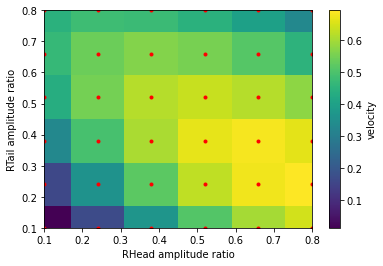
\includegraphics[height=0.3\columnwidth]{figures/8c_v1.png}
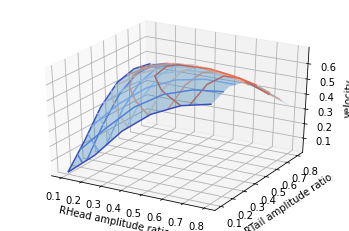
\includegraphics[height=0.3\columnwidth]{figures/8c_v2.png}
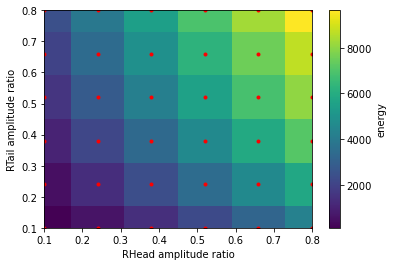
\includegraphics[height=0.3\columnwidth]{figures/8c_e1.png}
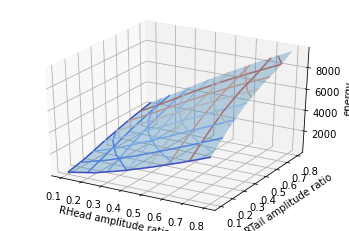
\includegraphics[height=0.3\columnwidth]{figures/8c_e2.png}
\caption{Grid search of amplitudes of the first and last oscillator, and their influence on speed (up) and energy (down)}
\label{c}
\end{figure}

The results of grid search are shown in Figure 14.
From the upper left corner of the Figure 14 we can observe that there is a certain head amplitude corresponding to the maximum velocity at each fixed tail amplitude. Before this point, the velocity increases with the increase of head amplitude. But the inverse trend appears after this point. The same phenomenon is observed when we fix the head amplitude and vary tail amplitude. If we connect the points corresponding to the maximum velocity at different amplitudes, we can find that the two amplitude coordinates of the maximum velocity are highly correlated, almost a straight line. The the velocity is symmetrically arranged on both sides of the line. The upper right corner of Figure 14 also shows that the maximum velocity occurs where the surface gradient is 0.

The lower left corner of Figure 14 also shows that the energy increases with the increase of both the amplitude of the head or tail. This paves a way reduce energy by reducing both amplitudes. The upper left corner of the Figure 14 illustrates that the point (parameters of both tail and head amplitudes) of maximum velocity does not necessarily correspond to the point of maximum energy, because the amplitude of tail corresponding to the maximum velocity is relatively small.


In the motion of a true salamander, the amplitude of one side of the whole body is increased from head to tail. This makes the head more stable and helps the visual system to observe and track prey as well as navigate. The tail, especially the part without limbs,
%(new improvement of Robotica samamandera 2), 
can move with a much larger amplitude because there is no coupling with the limbs. Decreasing the head amplitude and increasing the tail amplitude can increase the speed. While reducing the amplitude of the head with high mass and maintaining the high amplitude of the tail with low mass is beneficial to save energy.



\subsection*{8d. Turning and backwards swimming}
\label{sec:turning-backwards}

\begin{enumerate}
\item How do you need to modulate the CPG network (\corr{network.py}) in order
  to induce turning?  Implement this in the model and plot example GPS
  trajectories and spine angles.
\item How could you let the robot swim backwards? Explain and plot example GPS
  trajectories and spine angles.
\end{enumerate}

\begin{figure}[H]
\centering
\begin{tabular}{cc}
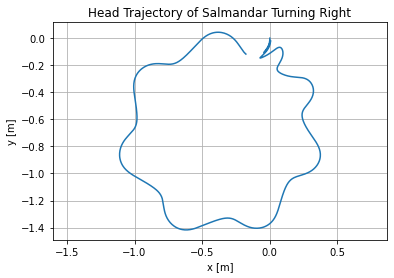
\includegraphics[height=0.3\columnwidth]{figures/8d_turn_traj_2.png} &
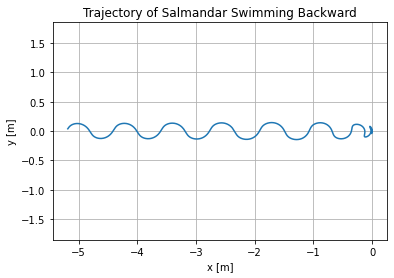
\includegraphics[height=0.3\columnwidth]{figures/8d_back_traj.png} \\
\textbf{(a)} & \textbf{(c)} \\
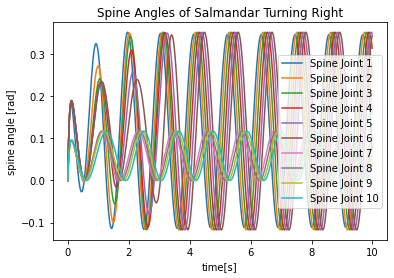
\includegraphics[height=0.3\columnwidth]{figures/8d_turn_spine_2.png} &
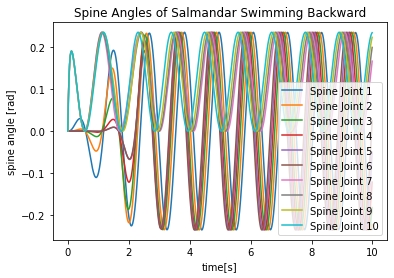
\includegraphics[height=0.3\columnwidth]{figures/8d_back_spine.png} \\
\textbf{(b)} & \textbf{(d)}
\end{tabular}
\caption{Spine angles plots with time along with position coordinates evolution for both turning right and swimming backwards.}
\label{c}
\end{figure}

To achieve turning (in our case, for instance, a right turn), one side of the spine should be triggered more than the other side. This can be easily realized through adding a turning parameter $\lambda$ to the amplitude of both sides of joints. The amplitudes of the joints can be modified as $r_{i}\times (1+\lambda)$
and $r_{i}\times (1-\lambda)$ so that we can set the value of $\lambda$ to have a biased joints amplitudes on 2 sides for a turning motion. In our simulation, we set $\lambda$ to 0.5 so that the spine movements always have a positive amplitude range. 
The phenomenon can be seen in Figure 15-(b) where the spine joint angles amplitudes are clearly varying in the positive direction only. This offset will cause the turning to the side receiving the larger amplitude variations. 

Changing the intrinsic frequency of some oscillators of axial leads to changes in the phase lags globally.
In moving forward, the first spine joint nearest to the head of the salamander has a phase lead over the other ones, and every subsequent joint leads the one after it, until the last joint at the tail of the salamander is reached. When a negative phase lag is applied, the first joint to jump into action would be Joint 10, as seen in Figure 15-(d). Then the previous joint is triggered, followed by the one before it, until reaching Joint 1 near the head. This will cause the salamander to start moving backwards. In simpler terms, simply reversing the directions (phase lag) of the joints for moving forward will cause the backward movement. Also, it can be observed through spine movements (d) that the tail joint leads the waves.
%What is worthy of mentioning is that from joints 7 to 10, the amplitude of the angle does not vary all the way from positive to negative values (unlike joints 1 to 6) but just oscillates in the positive region. This is the case since joint 7 is located at the rear limbs. That is, to achieve backward swimming, the salamander must move its upper body (from head to the rear limbs, i.e. joints 1 to 6) to give enough drive to push itself and swim backwards. Joints 7 to 10 can provide guidance (to move straight) and assistance in the drive backwards. 

To better show our turning and backward moving trend, we also recorded 2 videos and attached them in the folder.

\subsection*{8e. Cancelled}

\subsection*{8f. Limb – Spine coordination}
\label{sec:limb-spine-coordination}

In this next part you will explore the importance of a proper coordination
between the spine and the limb movement for walking.

\begin{enumerate}
\item Change the drive to a value used for walking and verify that the robot
  walks
\item Analyze the spine movement: What are your phase lags along the spine
  during walking? How does the spine movement compare to the one used for
  swimming?
\item Notice that the phase between limb and spine oscillators affects the
  robot’s walking speed. Run a parameter search on the phase offset between
  limbs and spine. Set the nominal radius R to 0.3 [rad]. Include plots showing
  how the phase offset influences walking speed and comment the results. How do
  your findings compare to body deformations in the salamander while walking?
\item Explore the influence of the oscillation amplitude along the body with
  respect to the walking speed of the robot. Run a parameter search on the
  nominal radius R with a fixed phase offset between limbs and the spine. For
  the phase offset take the optimal value from the previous sub-exercise. While
  exploring R, start from 0 (no body bending).
\end{enumerate}

Include plots showing how the oscillation radius influences walking speed and
comment on the results.

\begin{figure}[H]
\centering
\begin{tabular}{cc}
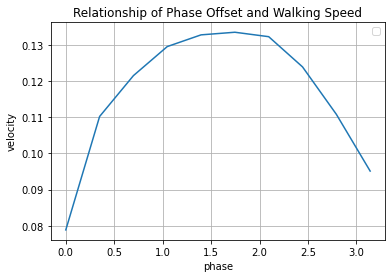
\includegraphics[height=0.3\columnwidth]{figures/8f_phase_3.png} &
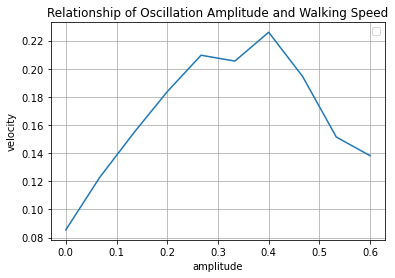
\includegraphics[height=0.3\columnwidth]{figures/8f_amp.png}   \\
\textbf{(a)} & \textbf{(b)}
\end{tabular}
\caption{Variation of walking speeds as a function of changing phase offsets and oscillation amplitudes.}
\label{c}
\end{figure}



During walking, a well-established in-sync coordination between the limbs and the spine is very important in achieving an optimal outcome when it comes to moving faster. Therefore, the element of phase lag introduced between the spine and the limbs becomes an important parameter that can be the difference between walking with maximum speed or maybe not walking at all. Here we set phase lag $0.2\pi$ between neighbour joints. The expected spine movement should conform to Figure \ref{a1} and Figure \ref{a2}.
%This is especially true for the case of spine joints 1 to 6, as they are the main key players in affecting the limbs directly. Spine joints 7 to 10 mainly affect the tail, a part not needed in walking. As such, spine joints 1 to 6 should exhibit an in-phase behavior among themselves while walking. In other words, the salamander body from head to rear limbs should be bending at the same time in the same manner. This results on no phase lag along the spine joints (1 to 6). Joints 7 to 10 exhibit an out-of-phase behavior with respect to joints 1 to 6.

In swimming, the limbs are no longer needed while the axial part becomes important in propagating the salamander in water. Having the whole body (from head to tail, i.e. all joints 1 to 10) be in oscillation becomes what is important in this process. Therefore, a phase lag between the spine and limb joints is no longer an important parameter. Rather, the phase lag along all the body spine joints themselves becomes crucial in moving while swimming. To move forward in this case, joint 1 must begin oscillating, followed by joint 2 after a very small delay, and so on until the last joint 10 is reached. This translates into having a propagating wave shape exhibited by the salamander body. This propagating wave allows the salamander to gain mobility in water. 

In walking standing wave there is no phase lag in both head part and the tail part of the spine while the head and tail have 2π difference of phase. In this case the phase offset between axial and limb is important. The maximum speed occurs when the body axial bends on the side of which the limbs stench forward (phase of the body). The bending curvature of the axial (amplitude of body oscillators) also influences the speed. While in swimming there is constant phase lags from the head to tail or from the tail to head. The total phase lag for both swimming and walking is 2π.

What follows will be comments on phase offset and oscillation amplitudes effects on the walking speed of the salamander. The velocity here is calculated through the final head joint's distance with respect to overall time.

In Figure 16-(a), generally the same velocity curve behavior is exhibited for a change in the phase offset given a fixed amplitude. An increase in the phase offset between body axial and limb of the salamander aids the walking process and allows for an increase in velocity. This increase reaches its maximum for a phase offset of around 1.4 rad. Afterwards, the velocity decreases with increase in phase. 

In Figure 16-(b), it is expected that for a fixed phase offset, as the amplitude of the body oscillations increases, the walking speed also increases. However, this is true up to a certain limit in amplitude (here around 0.4), after which the velocity decreases. This is expected since very big and out of control oscillations start to interfere with the limb movement, rendering it ineffective. 



Both figures show the importance of having a wave body motion along with the motion of the limbs to achieve higher speeds while walking. This is all under the condition that the phase offset and the amplitude of the oscillations do not bypass their respective threshold values providing highest efficiency for walking at higher speeds. Passing this threshold will put the body in an out-of-sync state with the limbs and will, in fact, render the walking process less efficient (having much lower speeds). 

\subsection*{8g. Land-to-water transitions}

\begin{enumerate}
\item In this exercise you will explore the gait switching mechanism. The gait
  switching is generated by a high level drive signal which interacts with the
  saturation functions that you should have implemented in 8a. Implement a new
  experiment which uses the x-coordinate of the robot in the world retrieved
  from the GPS sensor reading (Check \corr{simulation.py} for an example on how
  to access the gps data). Based on the GPS reading,
  you should determine if the robot should walk (it’s on land) or swim (it
  reached water). Depending on the current position of the robot, you should
  modify the drive such that it switches gait appropriately.
\item Run the Pybullet simulation and report spine and limb angles, together with
  the x coordinate from the GPS signal. Record a video showing the transition
  from land to water and submit the video together with this report.
\item (BONUS) Achieve water-to-land transition. Report spine and limb angles,
  the x-coordinate of the GPS and record a video.
\end{enumerate}


\textbf{Hint:} Use the record options as shown in \corr{exercise\_example.py} to
easily record videos.

\begin{figure}[H]
\centering
\begin{tabular}{cc}
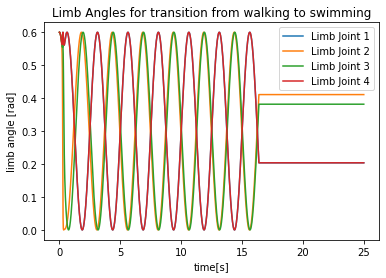
\includegraphics[height=0.3\columnwidth]{figures/8g_2_limb.png} &
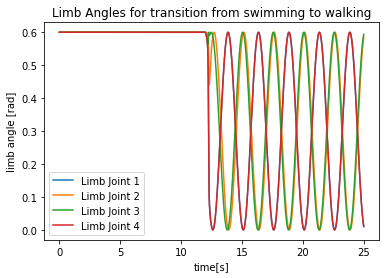
\includegraphics[height=0.3\columnwidth]{figures/8g_3_limb.png} \\
\textbf{(a)} & \textbf{(d)} \\
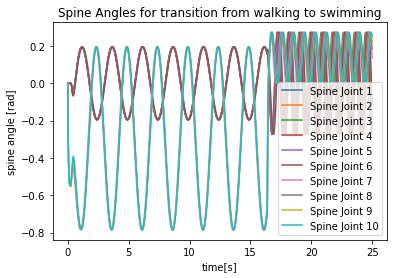
\includegraphics[height=0.3\columnwidth]{figures/8g_2_spine.png} &
\includegraphics[height=0.3\columnwidth]{figures/8g_3_spine.png} \\
\textbf{(b)} & \textbf{(e)} \\
\includegraphics[height=0.3\columnwidth]{figures/8g_2_x.png} &
\includegraphics[height=0.3\columnwidth]{figures/8g_3_x.png} \\
\textbf{(c)} & \textbf{(f)}
\end{tabular}
\caption{Plots for limb angles, spine angles, and x-position evolution with time when transitioning from walking to swimming. Same plots are shown also for the transition from swimming to walking.}
\label{c}
\end{figure}

Increasing the drive the motion of salamander shifted from walking to swimming and there is no overlap between the drive frequency for swimming and walking. 
The transition can be realized through changing the drive and other parameters that can directly help change the motion pattern. The condition for transition is based on the x-coordinate of the robot's head joint position. In our simulation, the land-to-water transition is realized by changing drive from 2 to 4 when head x  position is detected less than -2.2, while water-to-land transition is realized by changing drive from 3.5 to 2 when head x position is detected larger than -1.2.

As expected, in Figure 17-(a), the four limb joints behave in an oscillatory manner in while walking forward. Once the limb joints angles get fixed to a constant value, this is when swimming starts, as swimming does not require the motion of the limbs. In Figure 17-(b), the transition is clear at the same time stamp seen in limb angles figure before. These observations all conform to the analysis of swimming and walking pattern in previous sections.
%The spine joints active in a useful manner while walking are joints 1 to 6 as they allow control of the body section having the limbs. Joints 7 to 10 present a very different, and much larger peak-to-peak amplitude. However, these control the tail, which is a component not needed in walking. Once the transition to swimming occurs, joints 7 to 10 amplitudes decrease as the tail is now used in swimming. 

For a transition from swimming to walking, the exact opposite of what was shown earlier occurs. This can be clearly seen in Figure 17-(d) and Figure 17-(e).  

Besides, our group also tried another method for the transition based on the x-coordinate of different joints. Based on more precise location of water-land border, we can assign different motion parameters to different joints. For example, the robot has half the body on land while the other half in water during water-to-land transition. The front joints will have parameters for walking pattern while the tail joints are assigned with parameters for swimming pattern. However, the transition strategy may lead to turning over due to lack of physical coordination. Therefore, the transition by previous simpler method has a more robust performance, and in the report we only visualize the performance of that method. 

The videos of land-to-water and water-to-land transition have been recorded and attached in the folder.
% \newpage

\bibliography{lab8}
\label{sec:references}
\bibliographystyle{ieeetr}


% \newpage

% \section*{APPENDIX}
% \label{sec:appendix}

\end{document}

%%% Local Variables:
%%% mode: latex
%%% TeX-master: t
%%% End: